\documentclass[final,t]{beamer}
\catcode`\@=11
\mode<presentation>
{
%  \usetheme{Warsaw}
%  \usetheme{Aachen}
%  \usetheme{Oldi6}
%  \usetheme{I6td}
  \usetheme{I6dv}
%  \usetheme{I6pd}
%  \usetheme{I6pd2}
}



\def\bold#1{\mbox {\bf #1}}\def \vc #1#2{\bold {#1}_{#2}}\def \bftil #1#2{\bold {\widetild #1}_{#2}}
\def\bea{ \begin{eqnarray}}
\def\eea{\end{eqnarray}}
\def\cref#1{(\ref {#1})}
\def\Let@{\relax\iffalse{\fi\let\\=\cr\iffalse}\fi}
\def\vspace@{\def\vspace##1{\noalign{\vskip##1 }}}
\def\mat{\left[\matrix} \def\endmat{\endmatrix\right]}
%\def\vspace@{\def\vspace##1{\noalign{\vskip##1 }}}
\def\matrix{\,\vcenter\bgroup\Let@\vspace@
    \normalbaselines
  \m@th\ialign\bgroup\hfil$##$\hfil&&\quad\hfil$##$\hfil\crcr
    \mathstrut\crcr\noalign{\kern-\baselineskip}}
\def\endmatrix{\crcr\mathstrut\crcr\noalign{\kern-\baselineskip}\egroup
\egroup\,}


% additional settings
\setbeamerfont{itemize}{size=\normalsize}
\setbeamerfont{itemize/enumerate body}{size=\normalsize}
\setbeamerfont{itemize/enumerate subbody}{size=\normalsize}

% additional packages
\usepackage{times}
\usepackage{amsmath,amsthm, amssymb, latexsym,epsfig}
\usepackage{exscale}
%\boldmath
\usepackage{booktabs, array}
%\usepackage{rotating} %sideways environment
\usepackage[brazil]{babel}
\usepackage[utf8]{inputenc}
\usepackage{natbib}
\usepackage{ragged2e}

\usepackage{subfigure}
\usepackage[orientation=landscape,size=custom,width=90,height=120,scale=1.15]{beamerposter}

\listfiles
\graphicspath{{figures/}}
% Display a grid to help align images
%\beamertemplategridbackground[1cm]



\title{\huge One century of data from Vassouras Magnetic Observatory (1915-2015)}


\author[Benevides, Bassrei]{Artur Benevides, Edwin Camacho*, Vitor Silveira, Israelli Rodrigo, Rodrigo Melhorato e Kátia Pinheiro}
\institute[ON-MCTIC]{Observatório Nacional}
\date[Nov , 2017]{Nov. 15 , 2017}


% abbreviations
\usepackage{xspace}
\makeatletter
\DeclareRobustCommand\onedot{\futurelet\@let@token\@onedot}
\def\@onedot{\ifx\@let@token.\else.\null\fi\xspace}
\def\eg{{e.g}\onedot} \def\Eg{{E.g}\onedot}
\def\ie{{i.e}\onedot} \def\Ie{{I.e}\onedot}
\def\cf{{c.f}\onedot} \def\Cf{{C.f}\onedot}
\def\etc{{etc}\onedot}
\def\vs{{vs}\onedot}
\def\wrt{w.r.t\onedot}
\def\dof{d.o.f\onedot}
\def\etal{{et al}\onedot}
\makeatother

%%%%%%%%%%%%%%%%%%%%%%%%%%%%%%%%%%%%%%%%%%%%%%%%%%%%%%%%%%%%%%%%%%%%%%%%%%%%%%%%%%%%%%%%%%%%%%%%%%%%%%%%%%%%
%%%%%%%%%%%%%%%%%%%%%%%%%%%%%%%%%%%%%%%%%%%%%%%%%%%%%%%%%%%%%%%%%%%%%%%%%%%%%%%%%%%%%%%%%%%%%%%%%%%%%%%%%%%%
\begin{document}

  \begin{columns}[t]
    \begin{column}{.66\linewidth}

%%%%%%%%%%%%%%%%%%%%%%%%%%%%%%%%%%%%%%%%%%%%%%%%%%%%%%%%%%%%%%%%%%%%%%%%%%%%%%%%%%%%%%%%%%%%%%%%%%%%%%%%%%%%
%%%%%%%%%%%%%%%%%%%%%%%%%%%%%%%%%% Primeira coluna %%%%%%%%%%%%%%%%%%%%%%%%%%%%%%%%%%%%%%%%%%%%%%%%%%%%%%%%%
%%%%%%%%%%%%%%%%%%%%%%%%%%%%%%%%%%%%%%%%%%%%%%%%%%%%%%%%%%%%%%%%%%%%%%%%%%%%%%%%%%%%%%%%%%%%%%%%%%%%%%%%%%%%
\begin{block}{Introduction}
\justifying	
 Vassouras Magnetic Observatory (VSS) was the first observatory in Brazil, starting its measurements in 1915. VSS plays an important role in monitoring of the magnetic field in the south hemisphere mainly because is located in region of Southern Atlantic Magnetic Anomaly (SAMA). VSS is part of the INTERMAGNET since 1999 because of its high data quality and transmission in real time.
 
 This work presents the history of VSS as well as the centennial dataset (1915-2015). We	explore the comparison of VSS data and results of IGRF model, present a day Solarquiet and storm data as well the main characteristics of the secular variation in	VSS and the possible geomagnetic jerks occurring in this period.	
		

	
\end{block}

\begin{block}{History (1915 - 2015)}
	
In 1915 the director Morris of the observatory choose the ideal place for installing of the Vassoura Magnetic Observatory.
	
	
	
\end{block}


\begin{columns}
	\begin{column}{.31\linewidth}
	
\begin{block}{}


\begin{itemize}
\justifying
		\item \bf{Least Square Method (LSM)}
\end{itemize}

\begin{itemize}
\justifying
		\item \bf{Fit by spline interpolation}
\end{itemize}
The secular variation of X,Y and Z compontents were fitted using an algorithm  of linear fit by spline method: 
	\[ f(x)= f(x_{n-1})+t_{n-1}(x-x_{n-1}), \\
	for x_{n-1} \le x \le x_{n} \]\\

\begin{itemize}
\justifying
		\item \bf{Root Means Square (RMS)}
\end{itemize}
We calculated the erro between the model IGRF and the data from VSS using RMS:
\[e_{RMS}=\frac{1}{N} \sqrt{\sum\limits_{i=1}^{N}(m_{i}-d_{i})^{2}}, 
\]
the RMS can be view in the legends of figures.
 
	
\end{block}	


\end{column}
%%%%%%%%%%%%%%%%%%%%%%%%%%%%%%%%%%%%%%%%%%%%%%%%%%%%%%%%%%%%%%%%%%%%%%%%%%%%%%%%%%%%%%%%%%%%%%%%%%%%%%%%%%%%%%%%%%%%%%%%%%%%
%%%%%%%%%%%%%%%%%%%%%%%%%%%%%%%%%%%%%%%%%%%%%%%%%%% Segunda coluna %%%%%%%%%%%%%%%%%%%%%%%%%%%%%%%%%%%%%%%%%%%%%%%%%%%%%%%%%
%%%%%%%%%%%%%%%%%%%%%%%%%%%%%%%%%%%%%%%%%%%%%%%%%%%%%%%%%%%%%%%%%%%%%%%%%%%%%%%%%%%%%%%%%%%%%%%%%%%%%%%%%%%%%%%%%%%%%%%%%%%%
\begin{column}{.31\linewidth}


\begin{block}{Sq and Storm days}
	\justifying
\begin{figure}
	\centering
	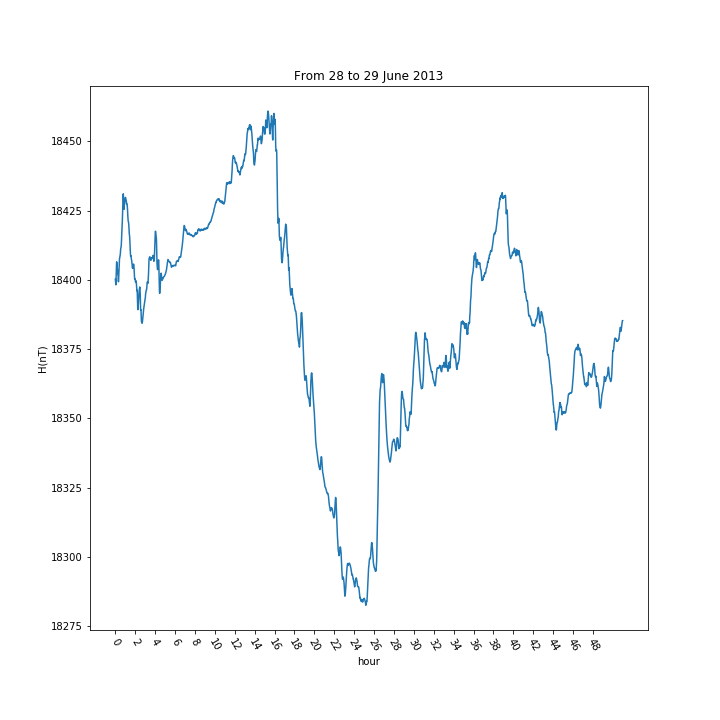
\includegraphics[width=0.6\linewidth]{28_29_june(2013)}
	\caption{8.}
	\label{storm}
\end{figure}	
	
\end{block}	
	

\end{column}


\begin{column}{.31\linewidth}
	
	
	\begin{block}{Geomagnetics Jerks}
		\justifying
		Possible ocurrence of geomagnetic jerks.
		
		Analyzing the X, Y and Z components:	
		\begin{figure}
			\centering
			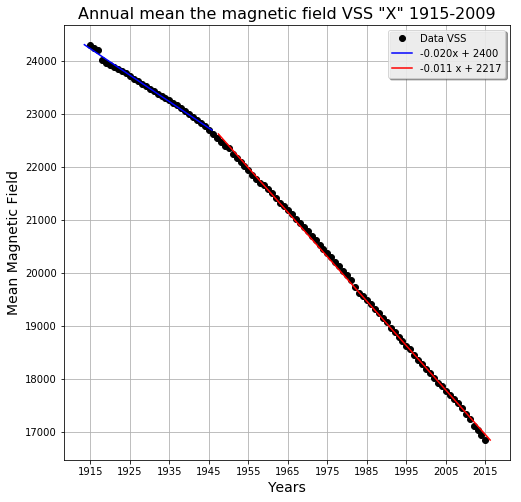
\includegraphics[width=0.6\linewidth]{retasX}
			\caption{9.}
			\label{w}
		\end{figure}	
		
		\begin{figure}
			\centering
			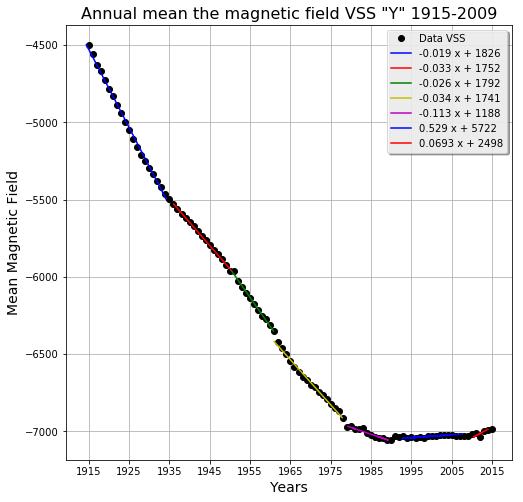
\includegraphics[width=0.6\linewidth]{retasY}
			\caption{10.}
			\label{fintetico}
		\end{figure}	
		
		
		\begin{figure}
			\centering
			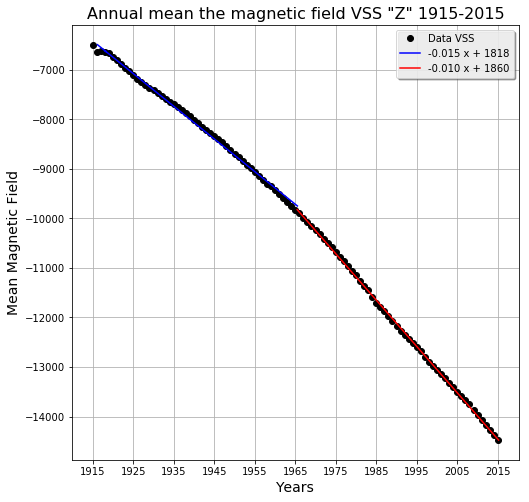
\includegraphics[width=0.6\linewidth]{retasZ}
			\caption{11.}
			\label{fig:g_Sintetico}
		\end{figure}

Analyzing the secular variations for spline fits: 		
		\begin{figure}
			\centering
			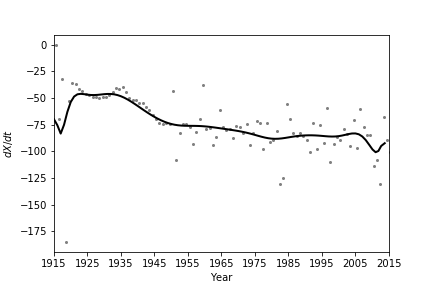
\includegraphics[width=0.7\linewidth]{spline101sv_X_spline}
			\caption{12. Secular variation to X component}
			\label{SPLINEx}
		\end{figure}
		
		\begin{figure}
			\centering
			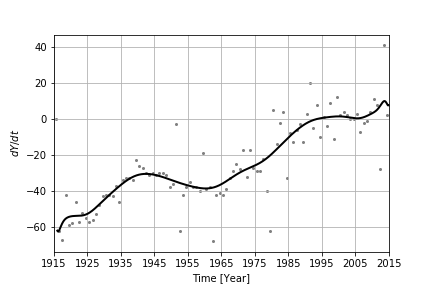
\includegraphics[width=0.7\linewidth]{spline100sv_y_spline}
			\caption{13. Secular variation to Y component.}
			\label{SPLINEy}
		\end{figure}
		
		\begin{figure}
			\centering
			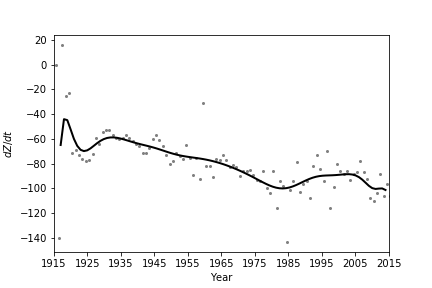
\includegraphics[width=0.7\linewidth]{spline100sv_z_spline}
			\caption{14 Secular variation to Z component.}
			\label{Splinez}
		\end{figure}
		
		
		
		
		
		
	\end{block}
\end{column}	

\end{columns}

\end{column}
%%%%%%%%%%%%%%%%%%%%%%%%%%%%%%%%%%%%%%%%%%%%%%%%%%%%%%%%%%%%%%%%%%%%%%%%%%%%%%%%%%%%%%%%%%%%%%%%%%%%%%%%%%%%
%%%%%%%%%%%%			Terceira Coluna %%%%%%%%%%%%%%%%%%%%%%%%%%%%%%%%%%%%%%%%%%%%%%%%%%%%%%%%%%%%%%%%%%%% %%%%%%%%%%%%							%%%%%%%%%%%%%%%%%%%%%%%%%%%%%%%%%%%%%%%%%%%%%%%%%%%%%%%%%%%%%%%%%%%%
%%%%%%%%%%%%%%%%%%%%%%%%%%%%%%%%%%%%%%%%%%%%%%%%%%%%%%%%%%%%%%%%%%%%%%%%%%%%%%%%%%%%%%%%%%%%%%%%%%%%%%%%%%%%
\begin{column}{.33\linewidth}


\begin{block}{VSS}
	\justifying
\begin{figure}
\centering
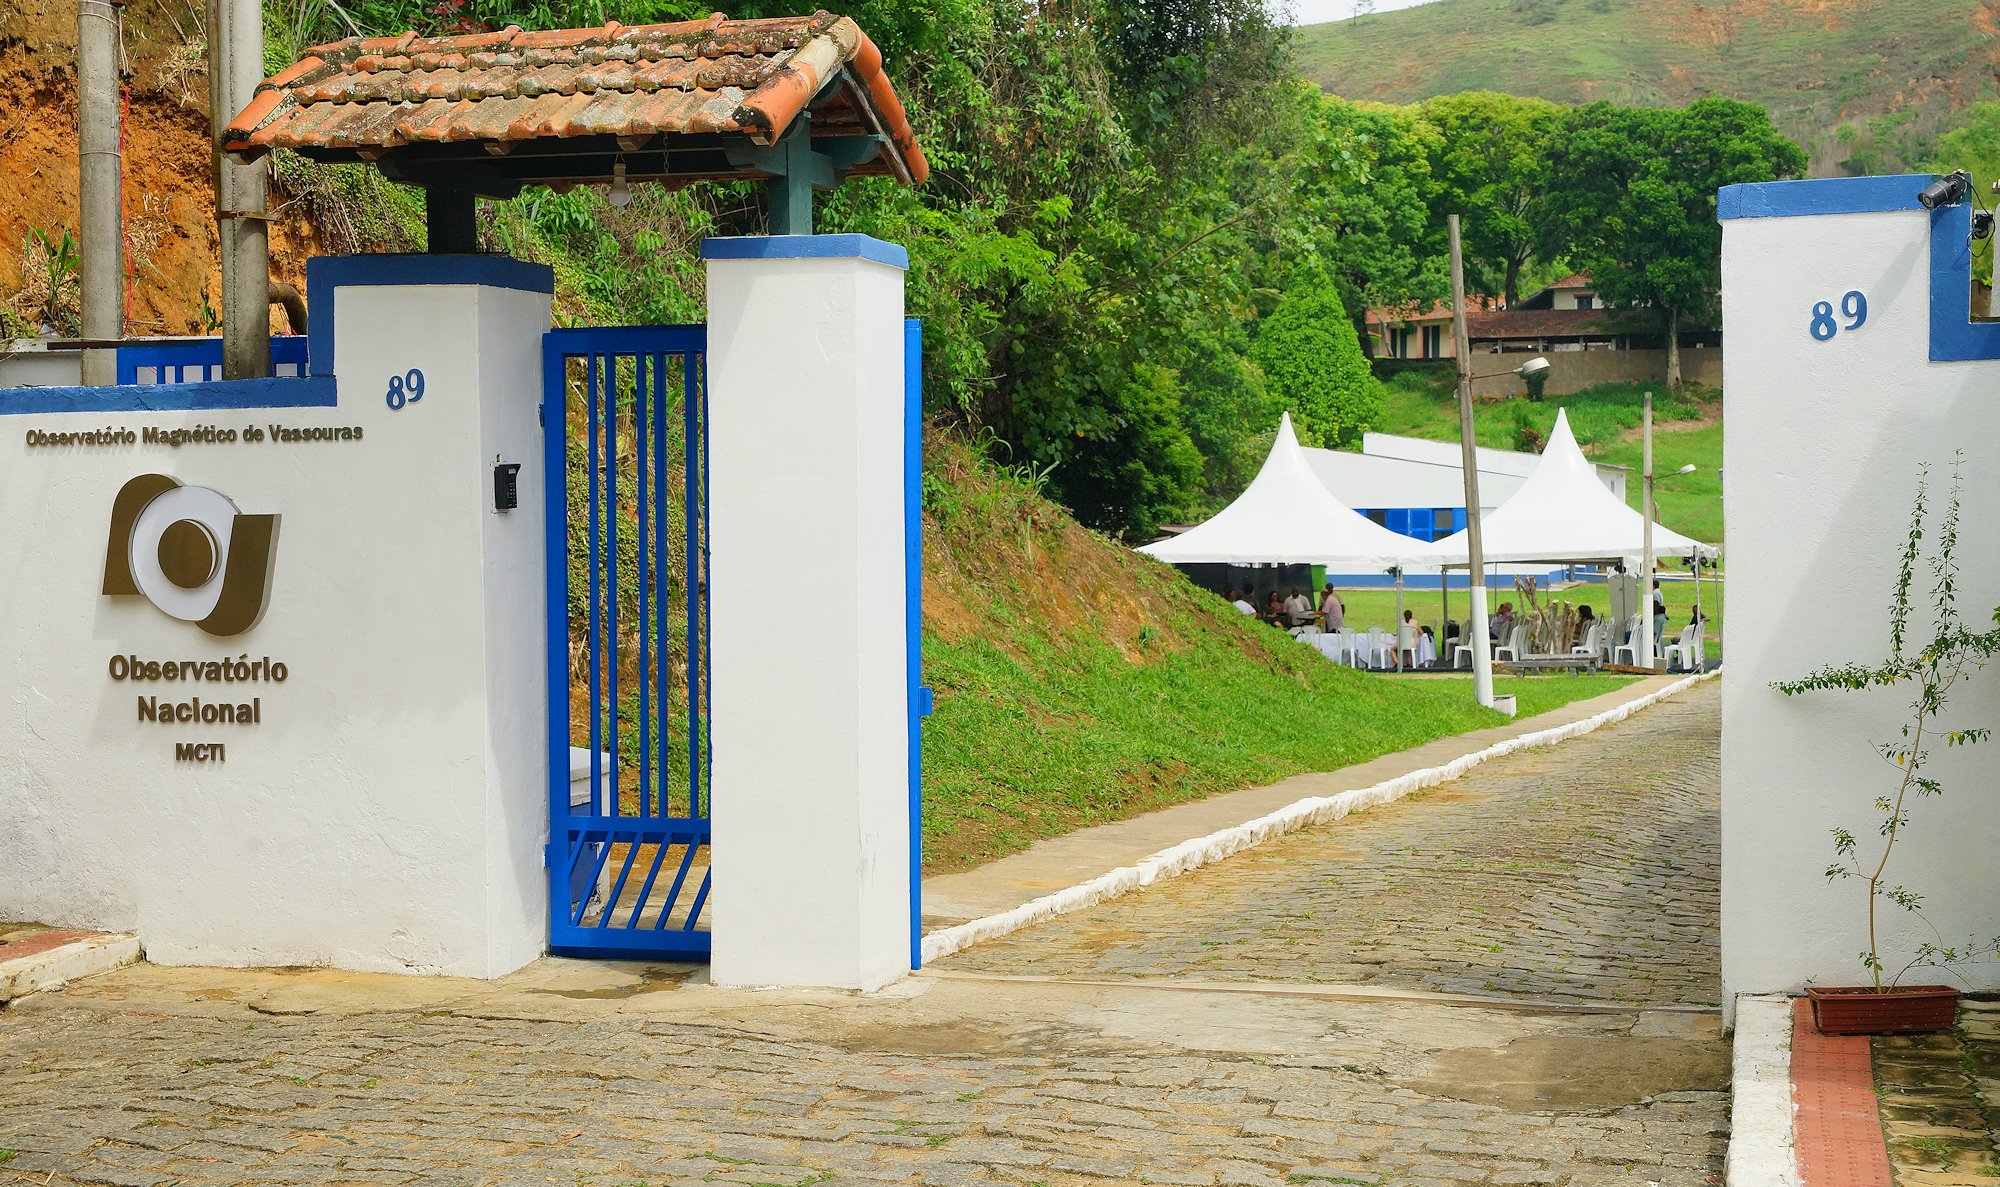
\includegraphics[width=0.7\linewidth]{OMV_JOELSONMOREIRA}
\caption{}
\label{fig:OMV_JOELSONMOREIRA}
\end{figure}





\end{block}

\begin{block}{VSS}
	\centering
\begin{tabular}{|c|c|c|c|}
		\hline
		\multicolumn{4}{|c|}{\textbf{Change/year}}\\	
	\hline   & VSS (nT)& IGRF12 (nT) & WMM2015 (nT)\\ 
	\hline Total intensity & -22,7  & -3.0  & -7.8  \\ 
	\hline X component & -74,7 & -98.0 & -93.3 \\ 
	\hline Y component & 24,9  & 2.2 & 5.4 \\ 
	\hline Z component & -79,8 & -91.6  & -94.1\\ 
	\hline H component  & -64,7 & -85.3 & -88.2\\ 
	\hline I component  & -0° 14' 13" & -0° 19' 15" &-0° 19' 5"\\ 
	\hline D component  & -0° 7' 2,28" & -0° 6' 25" & -0° 5' 59"\\ 
	\hline 
\end{tabular} 
	
	
	
	
	
\end{block}


%\begin{block}{References}
%\bibliographystyle{seg} 
%\bibliography{references}
%\end{block}



\begin{block}{Referencias}

\begin{itemize}
\item
\end{itemize}
\vspace{-0.2cm}
\end{block}

\end{column}

\end{columns}
\end{document}


%\begin{figure}
%%	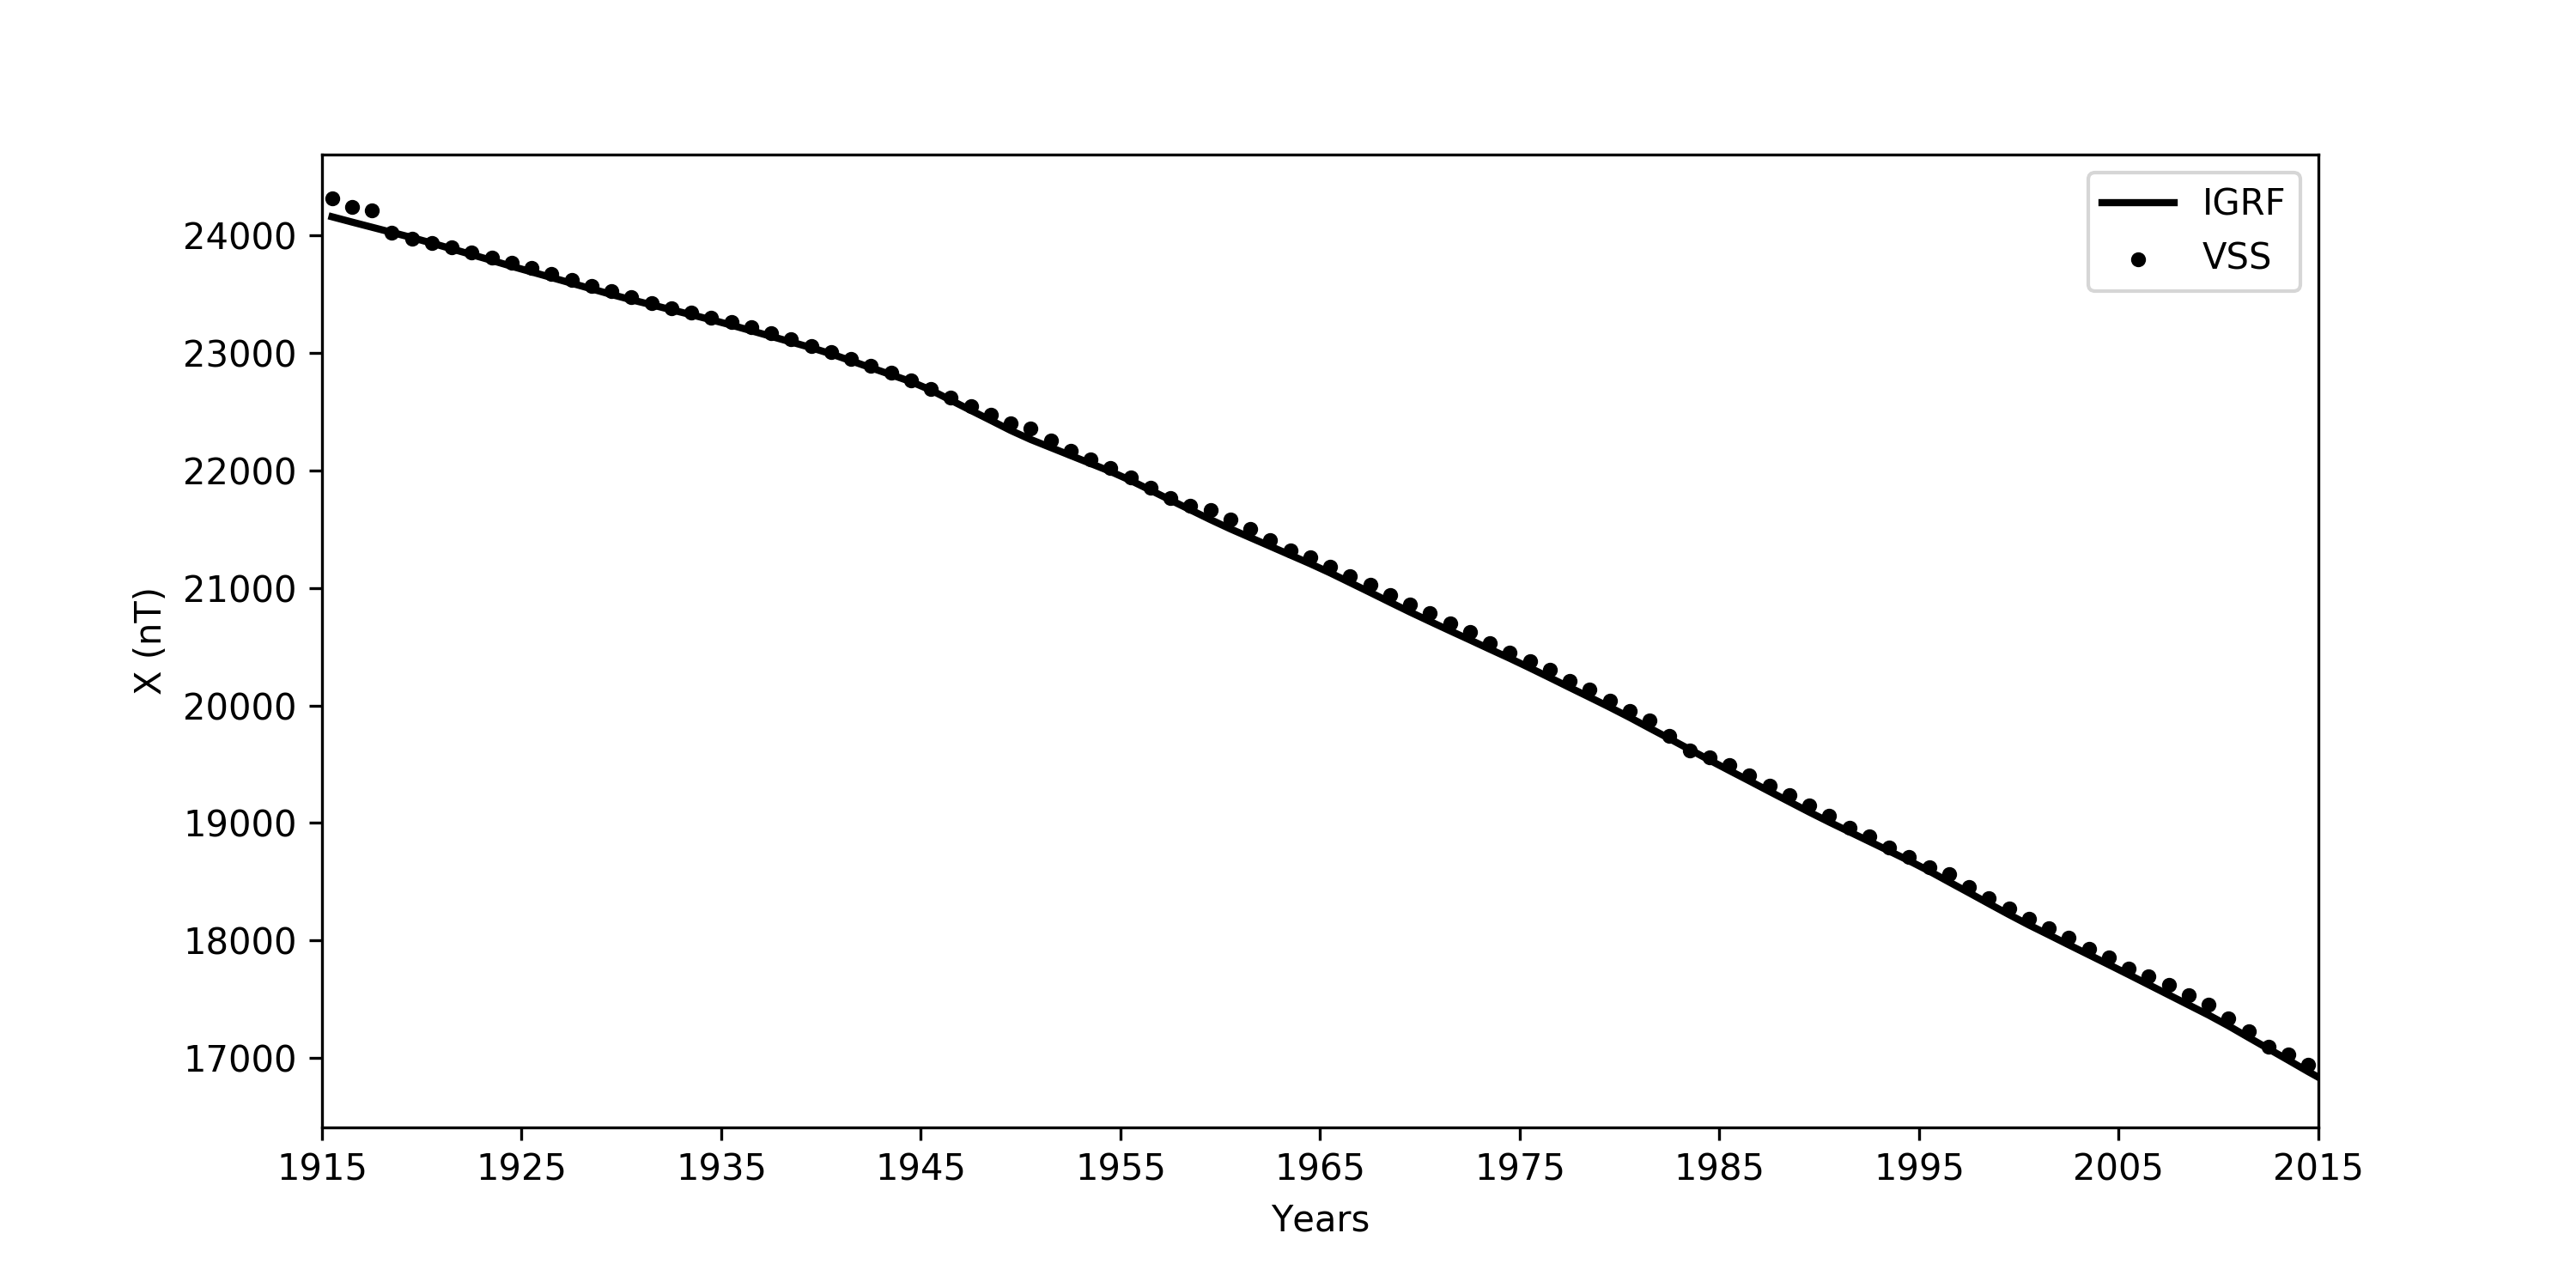
\includegraphics[width=1.0\linewidth]{X}
%	\caption{1. Root means square (RMS) between VSS data and IGRF model (X component) is 0.25 (\%)}
%	\label{X}
%\end{figure}

%\begin{figure}
%	\centering
%	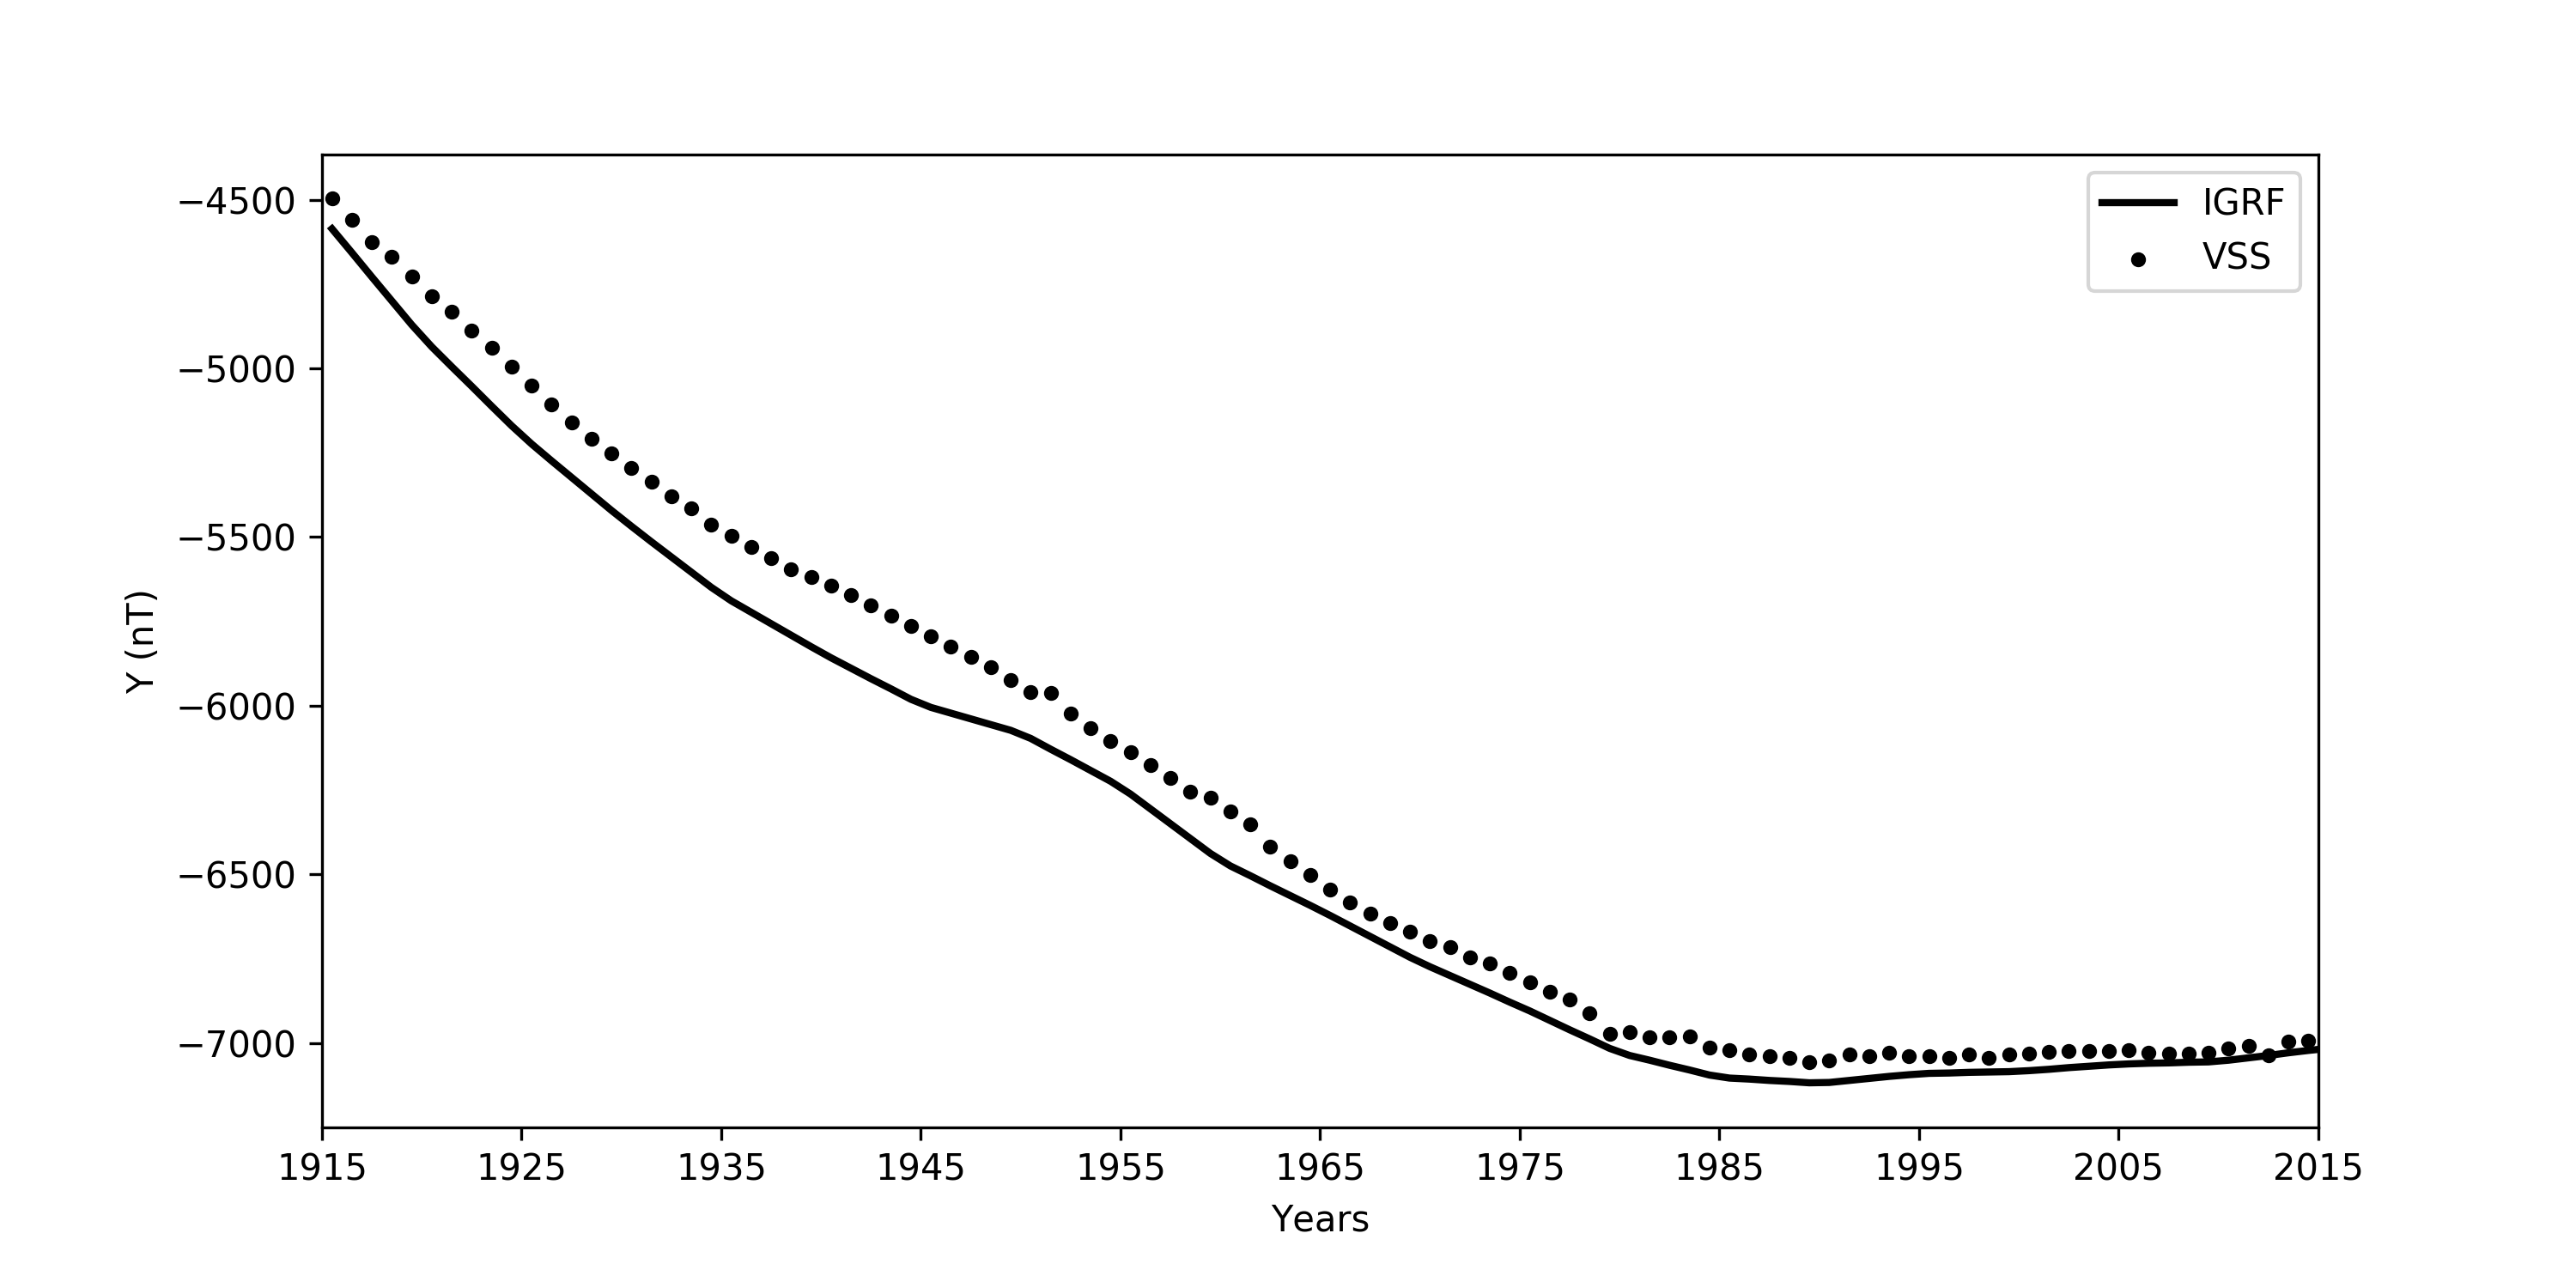
\includegraphics[width=1.0\linewidth]{Y}
%	\caption{2. RMS (Y component) = 1.98 (\%)}
%	\label{y}
%\end{figure}

%\begin{figure}
%	\centering
%	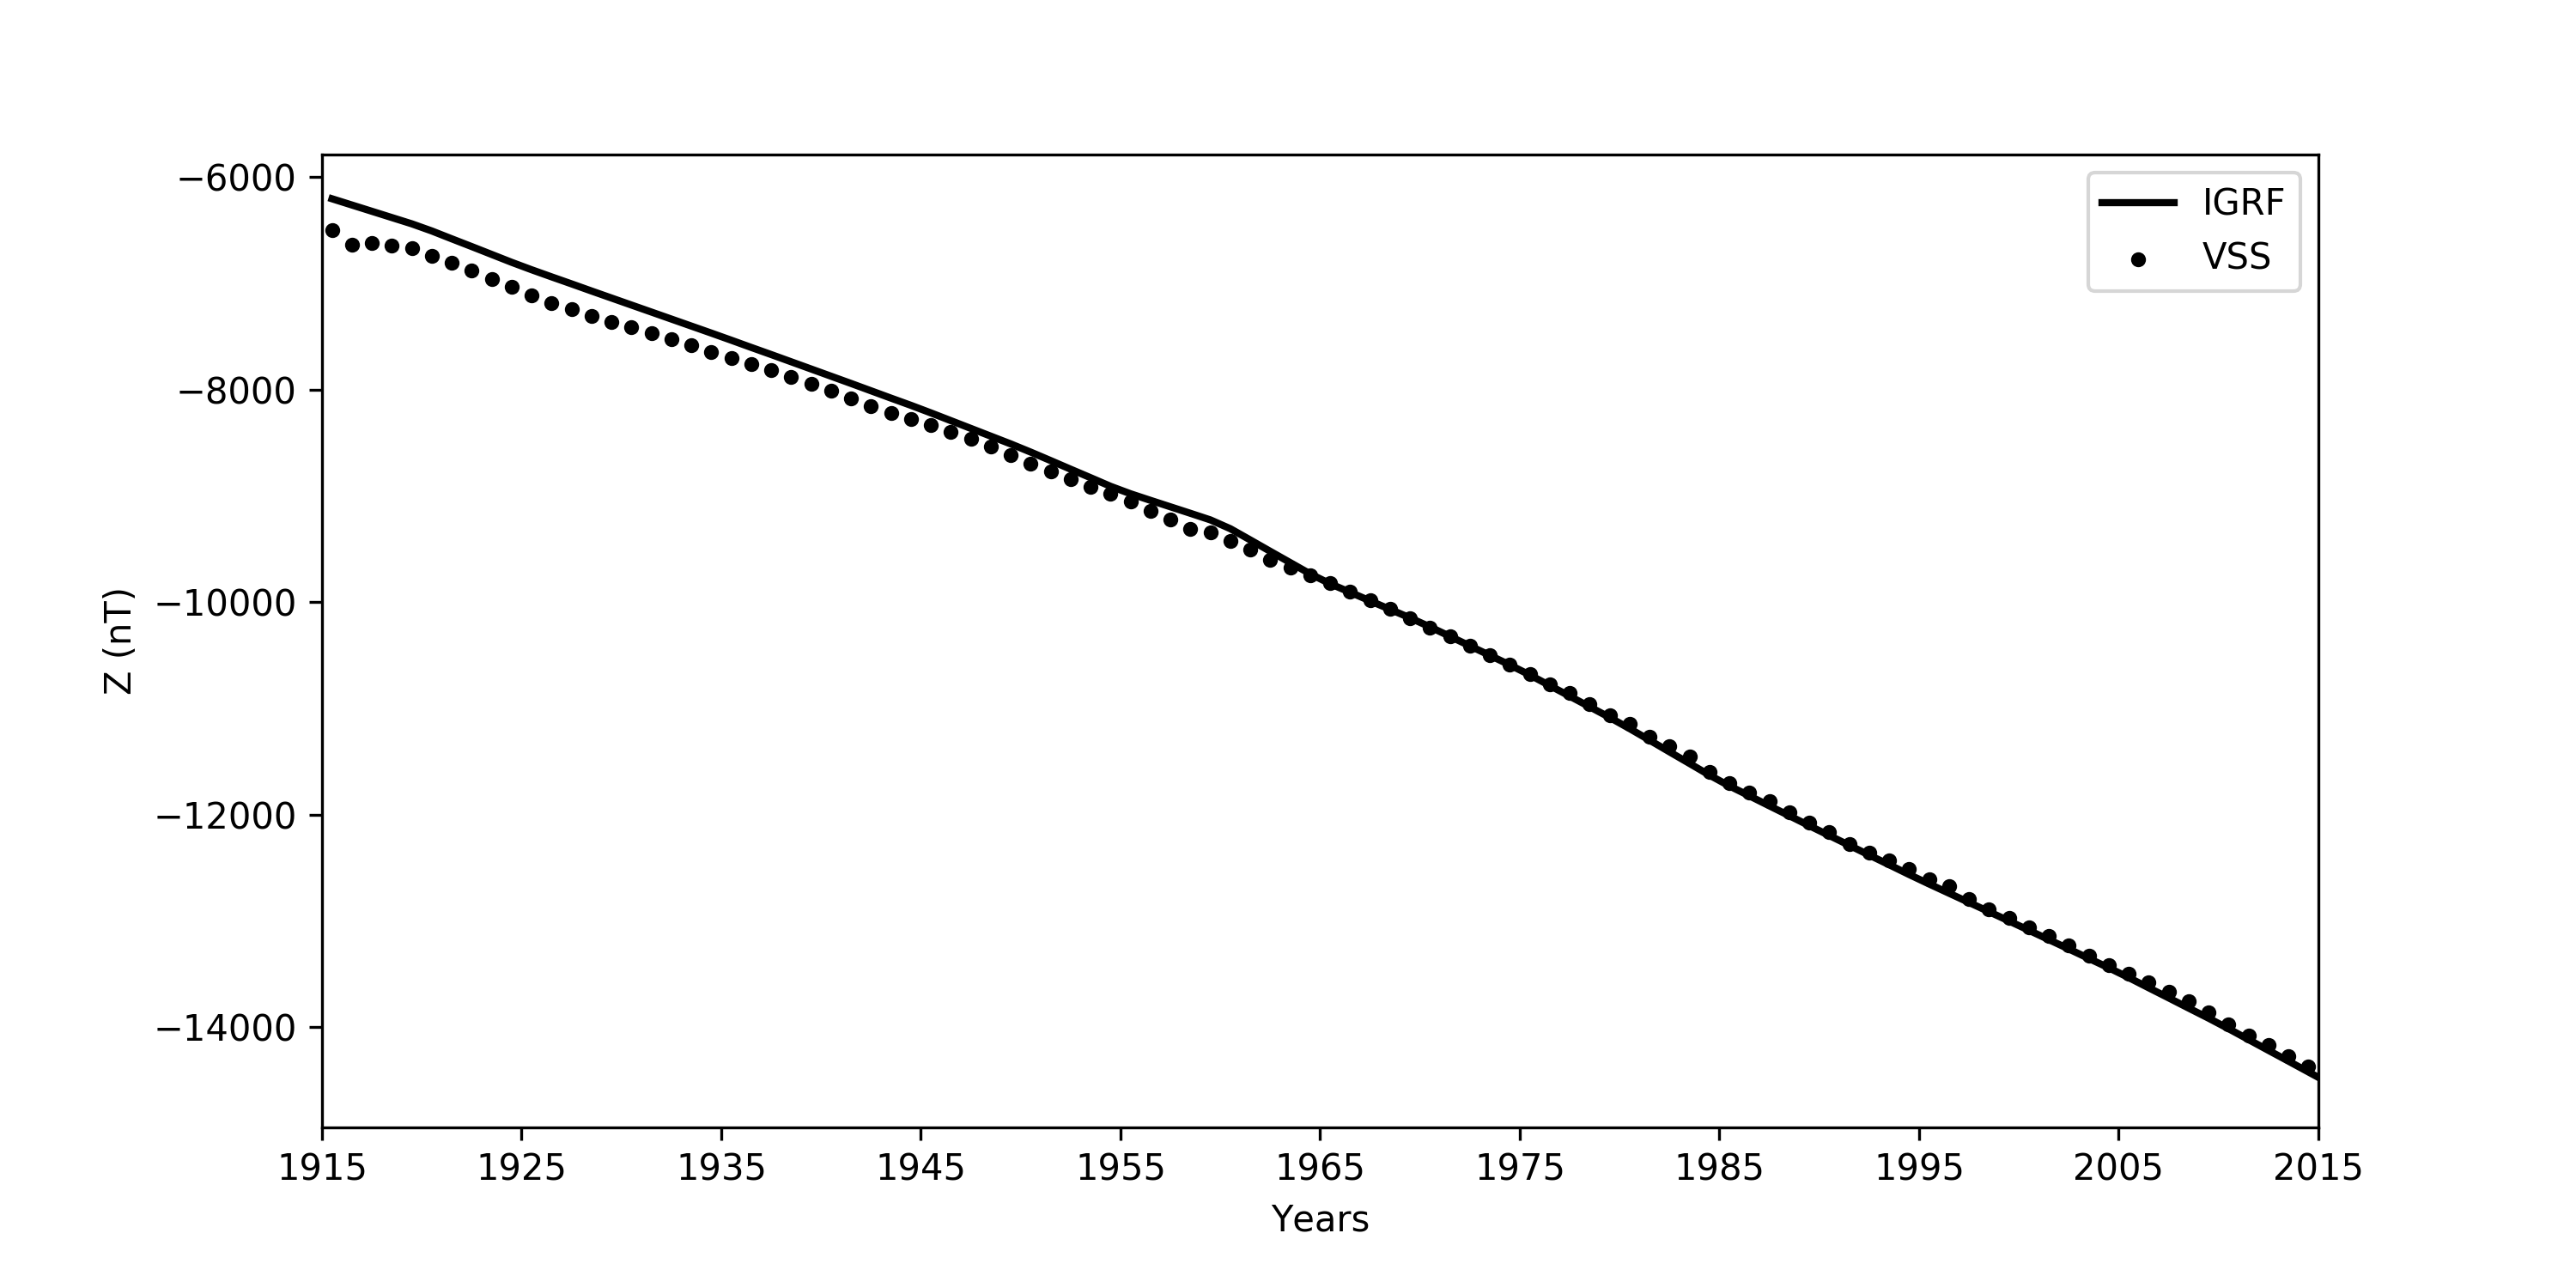
\includegraphics[width=1.0\linewidth]{Z}
%	\caption{3. RMS (Z component) = 1.22 (\%)}
%	\label{z}
%\end{figure}

%\begin{figure}
%	\centering
%	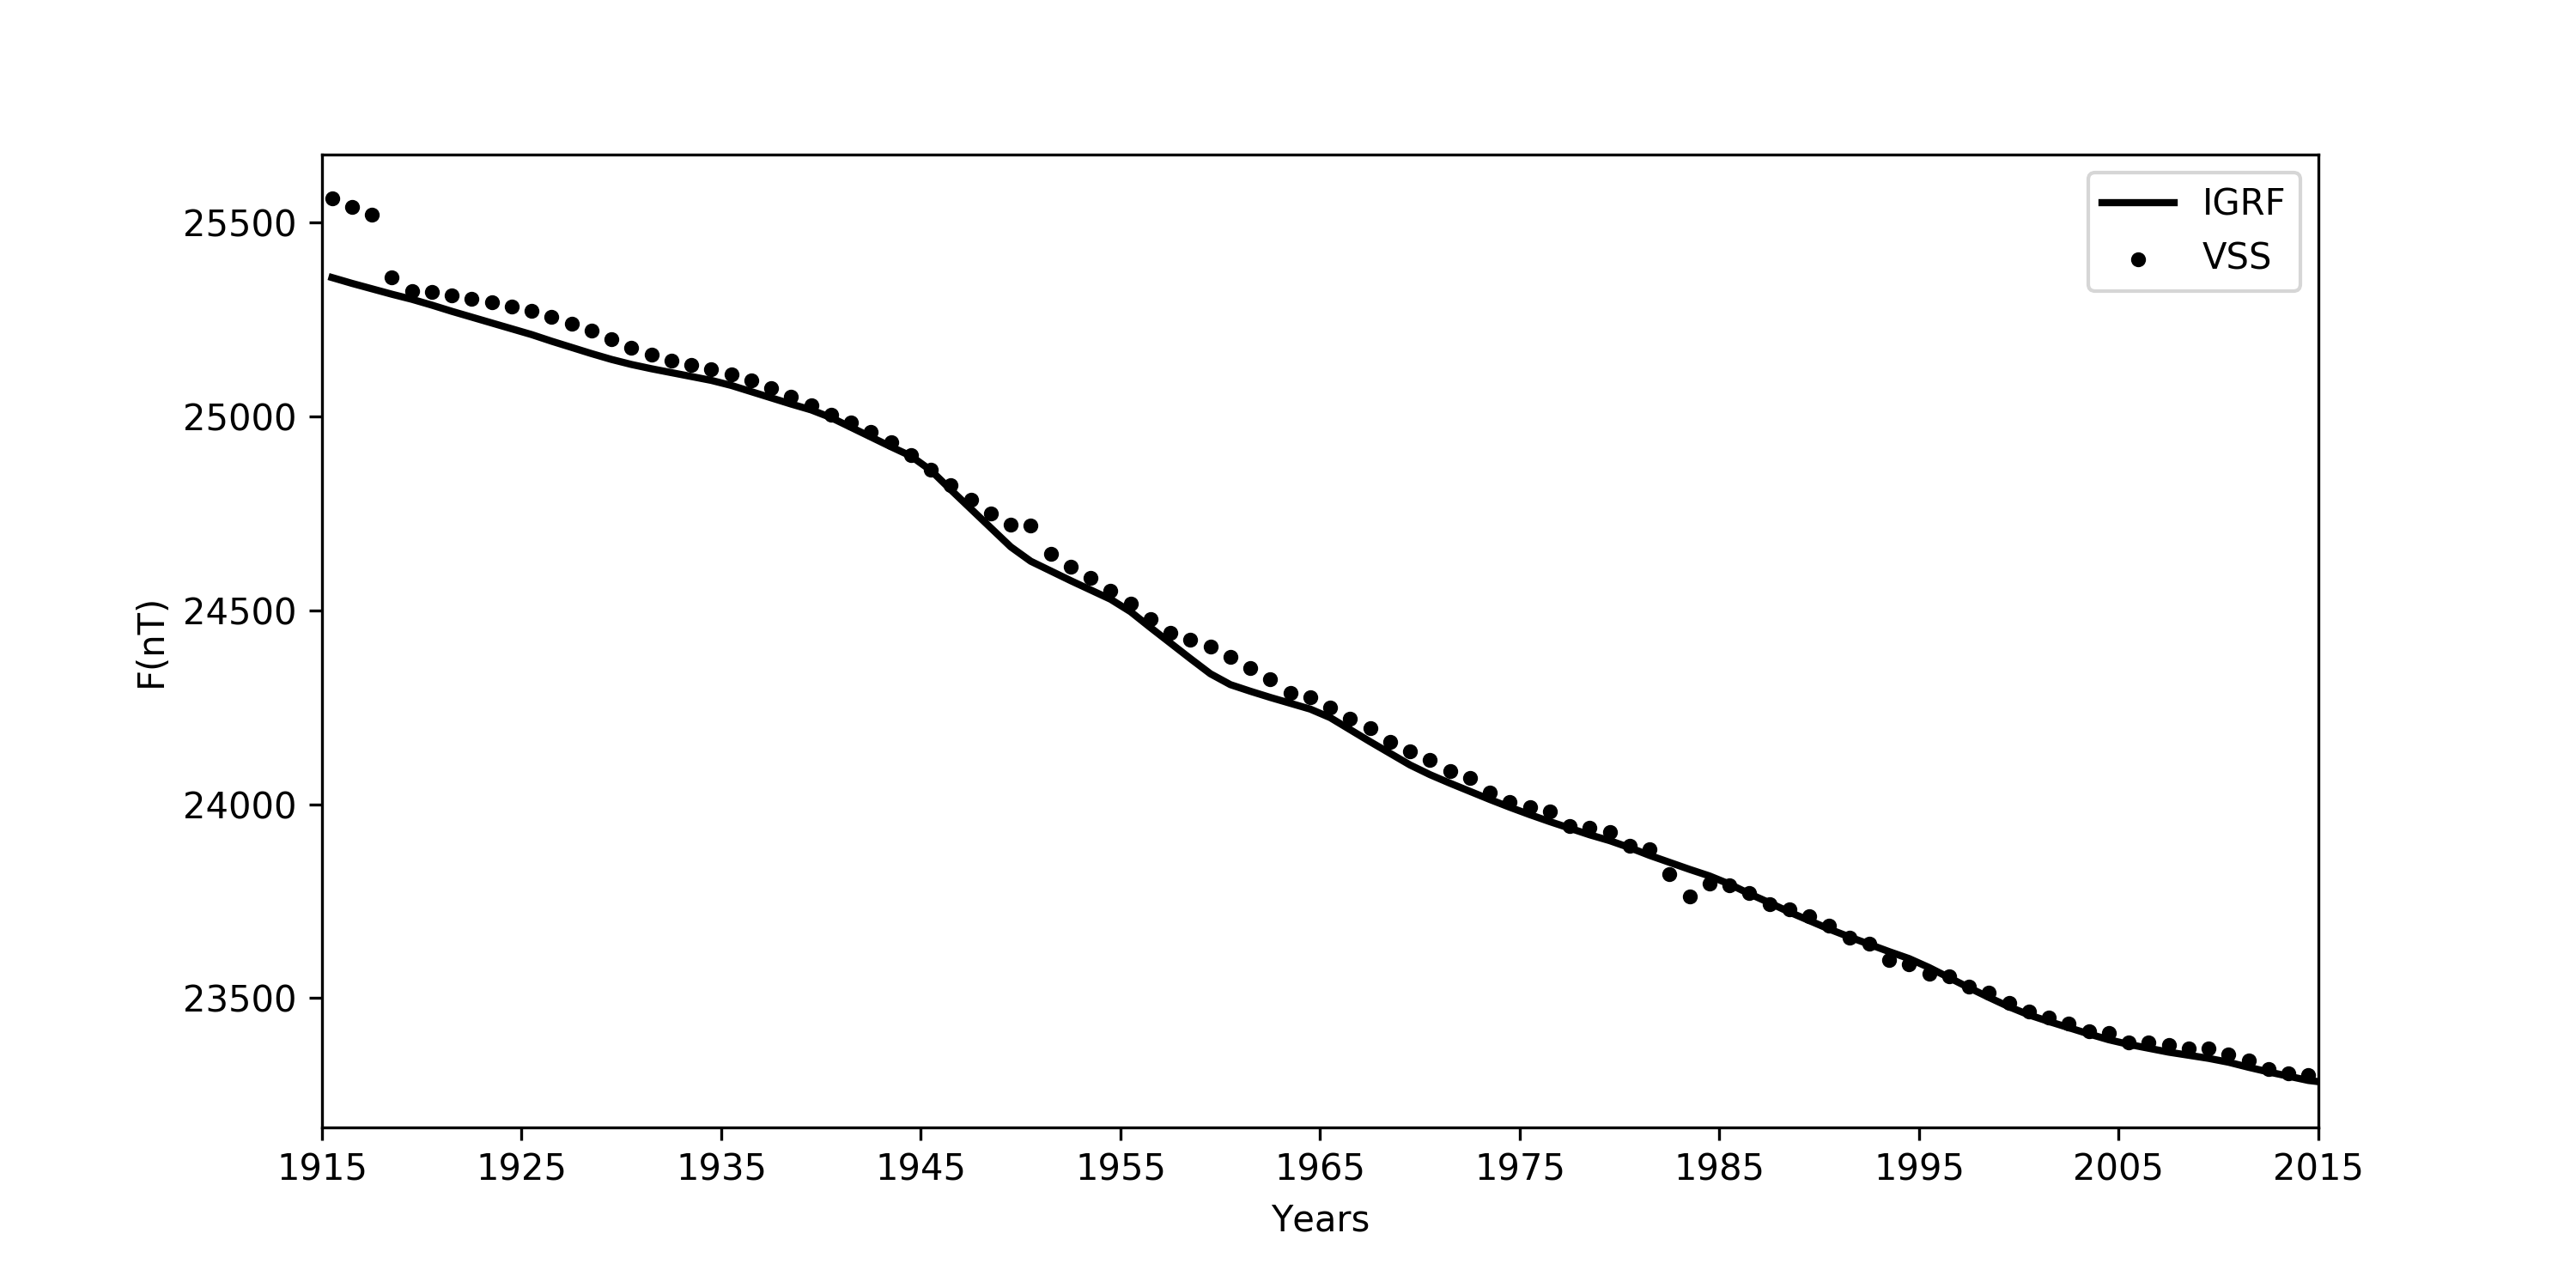
\includegraphics[width=1.0\linewidth]{F}
%	\caption{4. RMS (Intensity F) = 0.19 (\%)}
%	\label{f}
%\end{figure}



%\begin{figure}
%	\centering
%	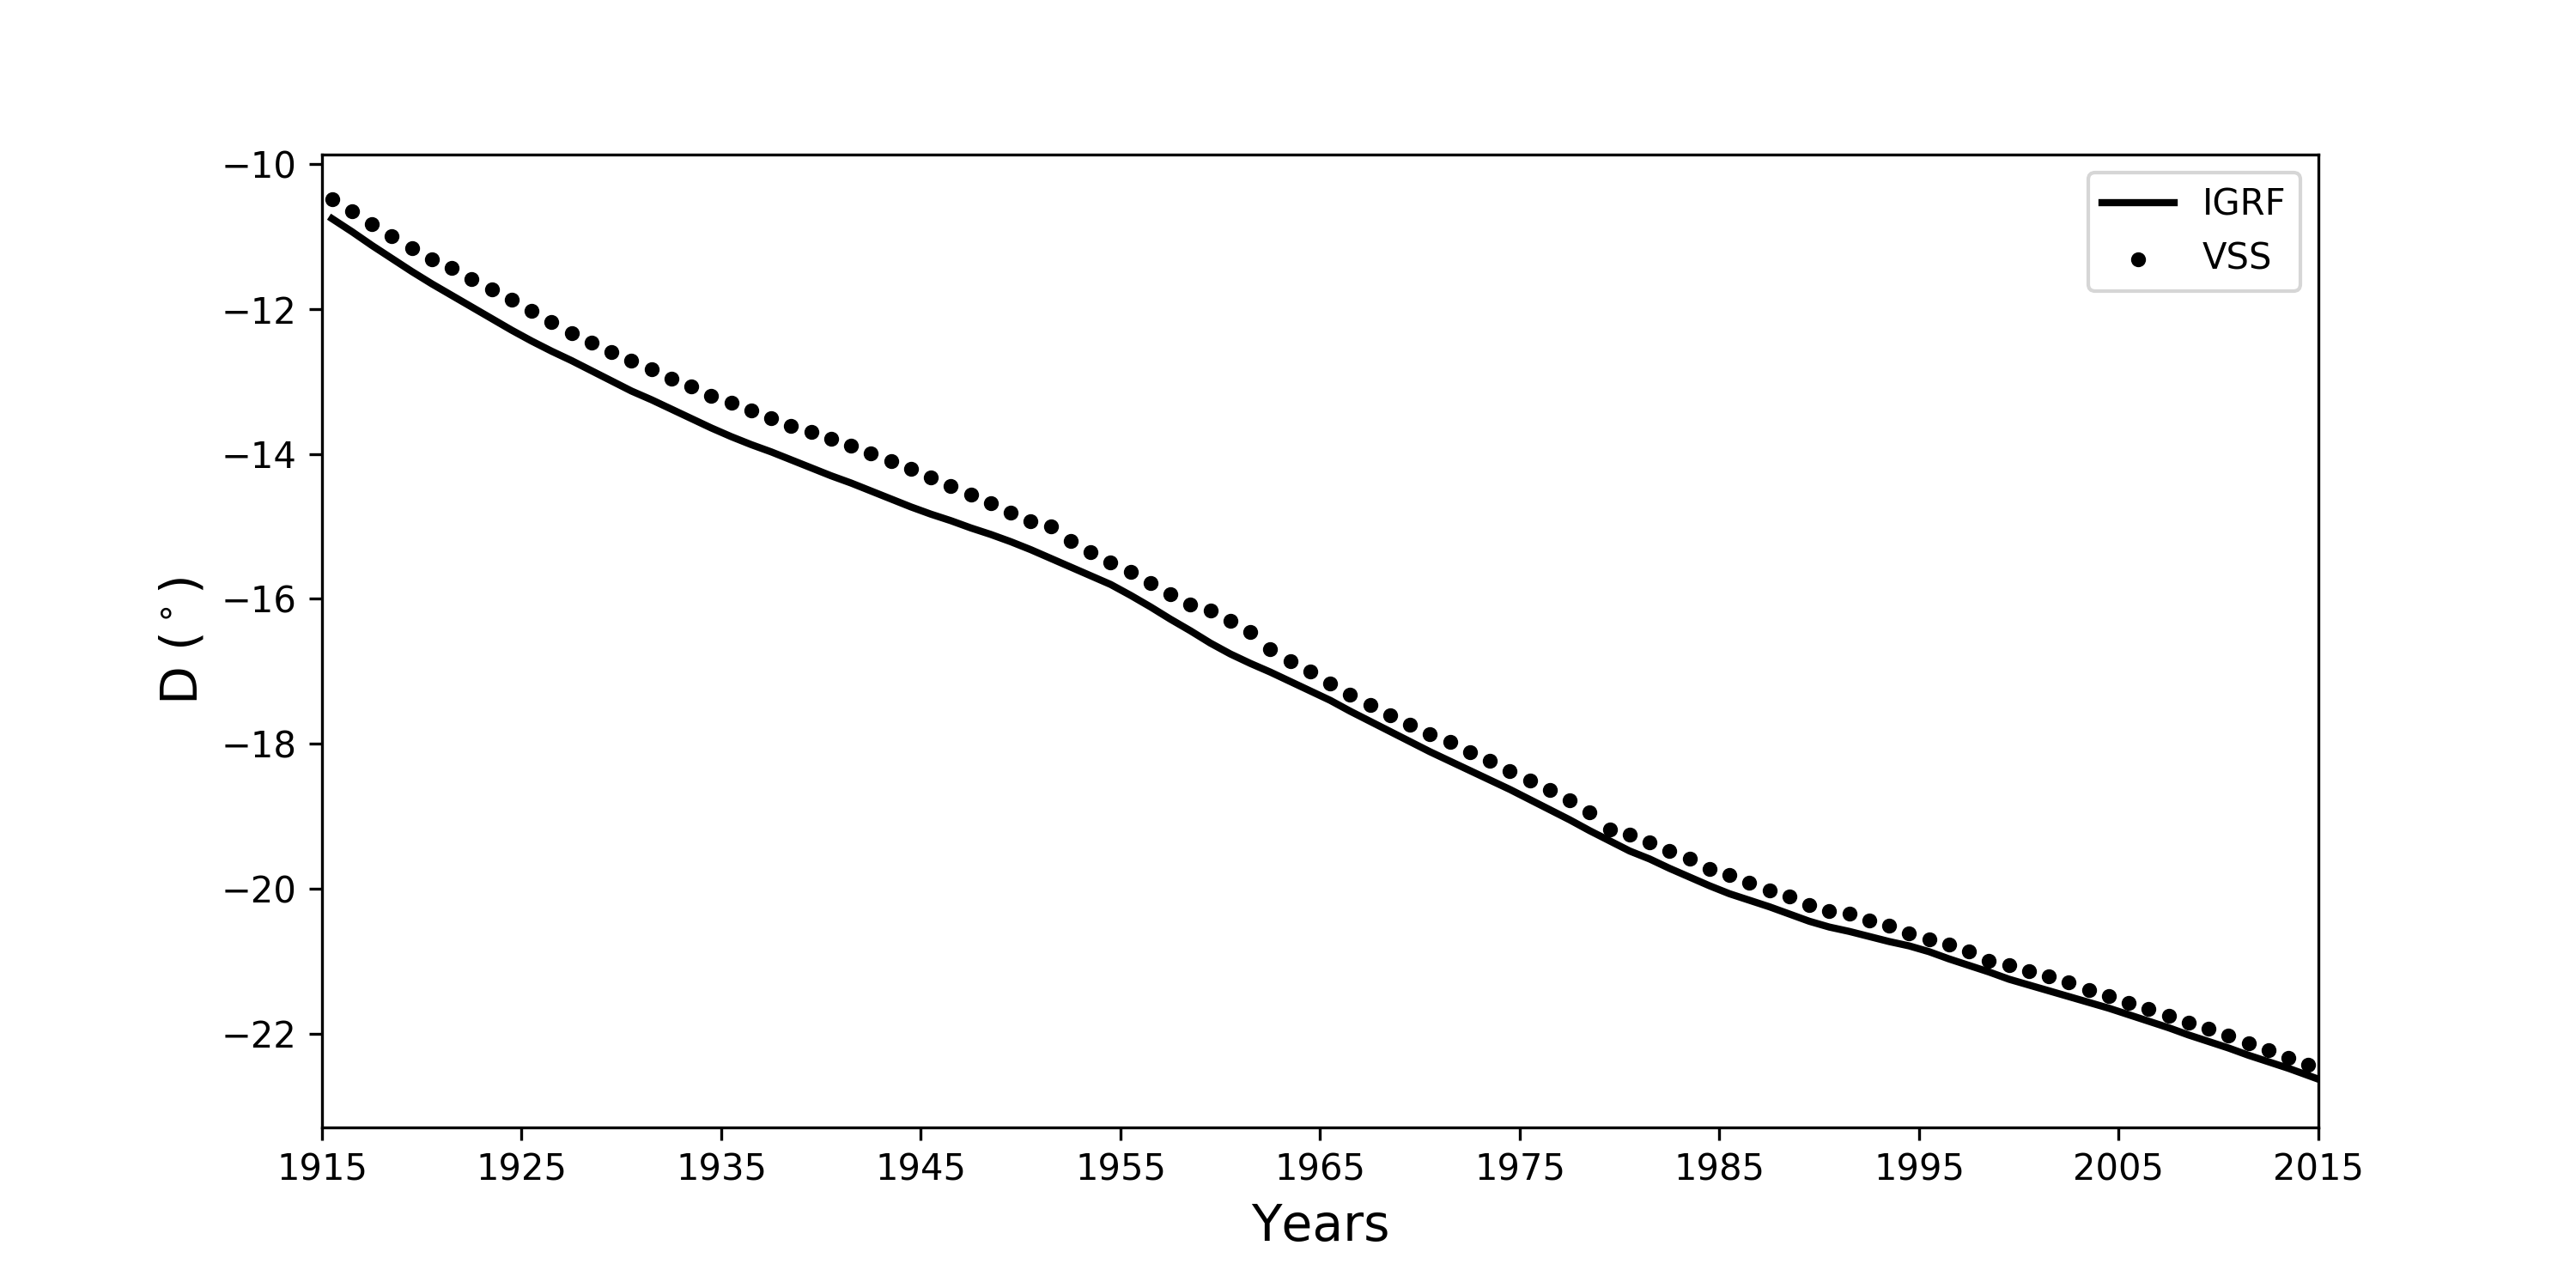
\includegraphics[width=1.0\linewidth]{D}
%	\caption{5. RMS (Inclination) = 1.1 (\%)}
%	\label{fo}
%\end{figure}


%\begin{figure}
%	\centering
%	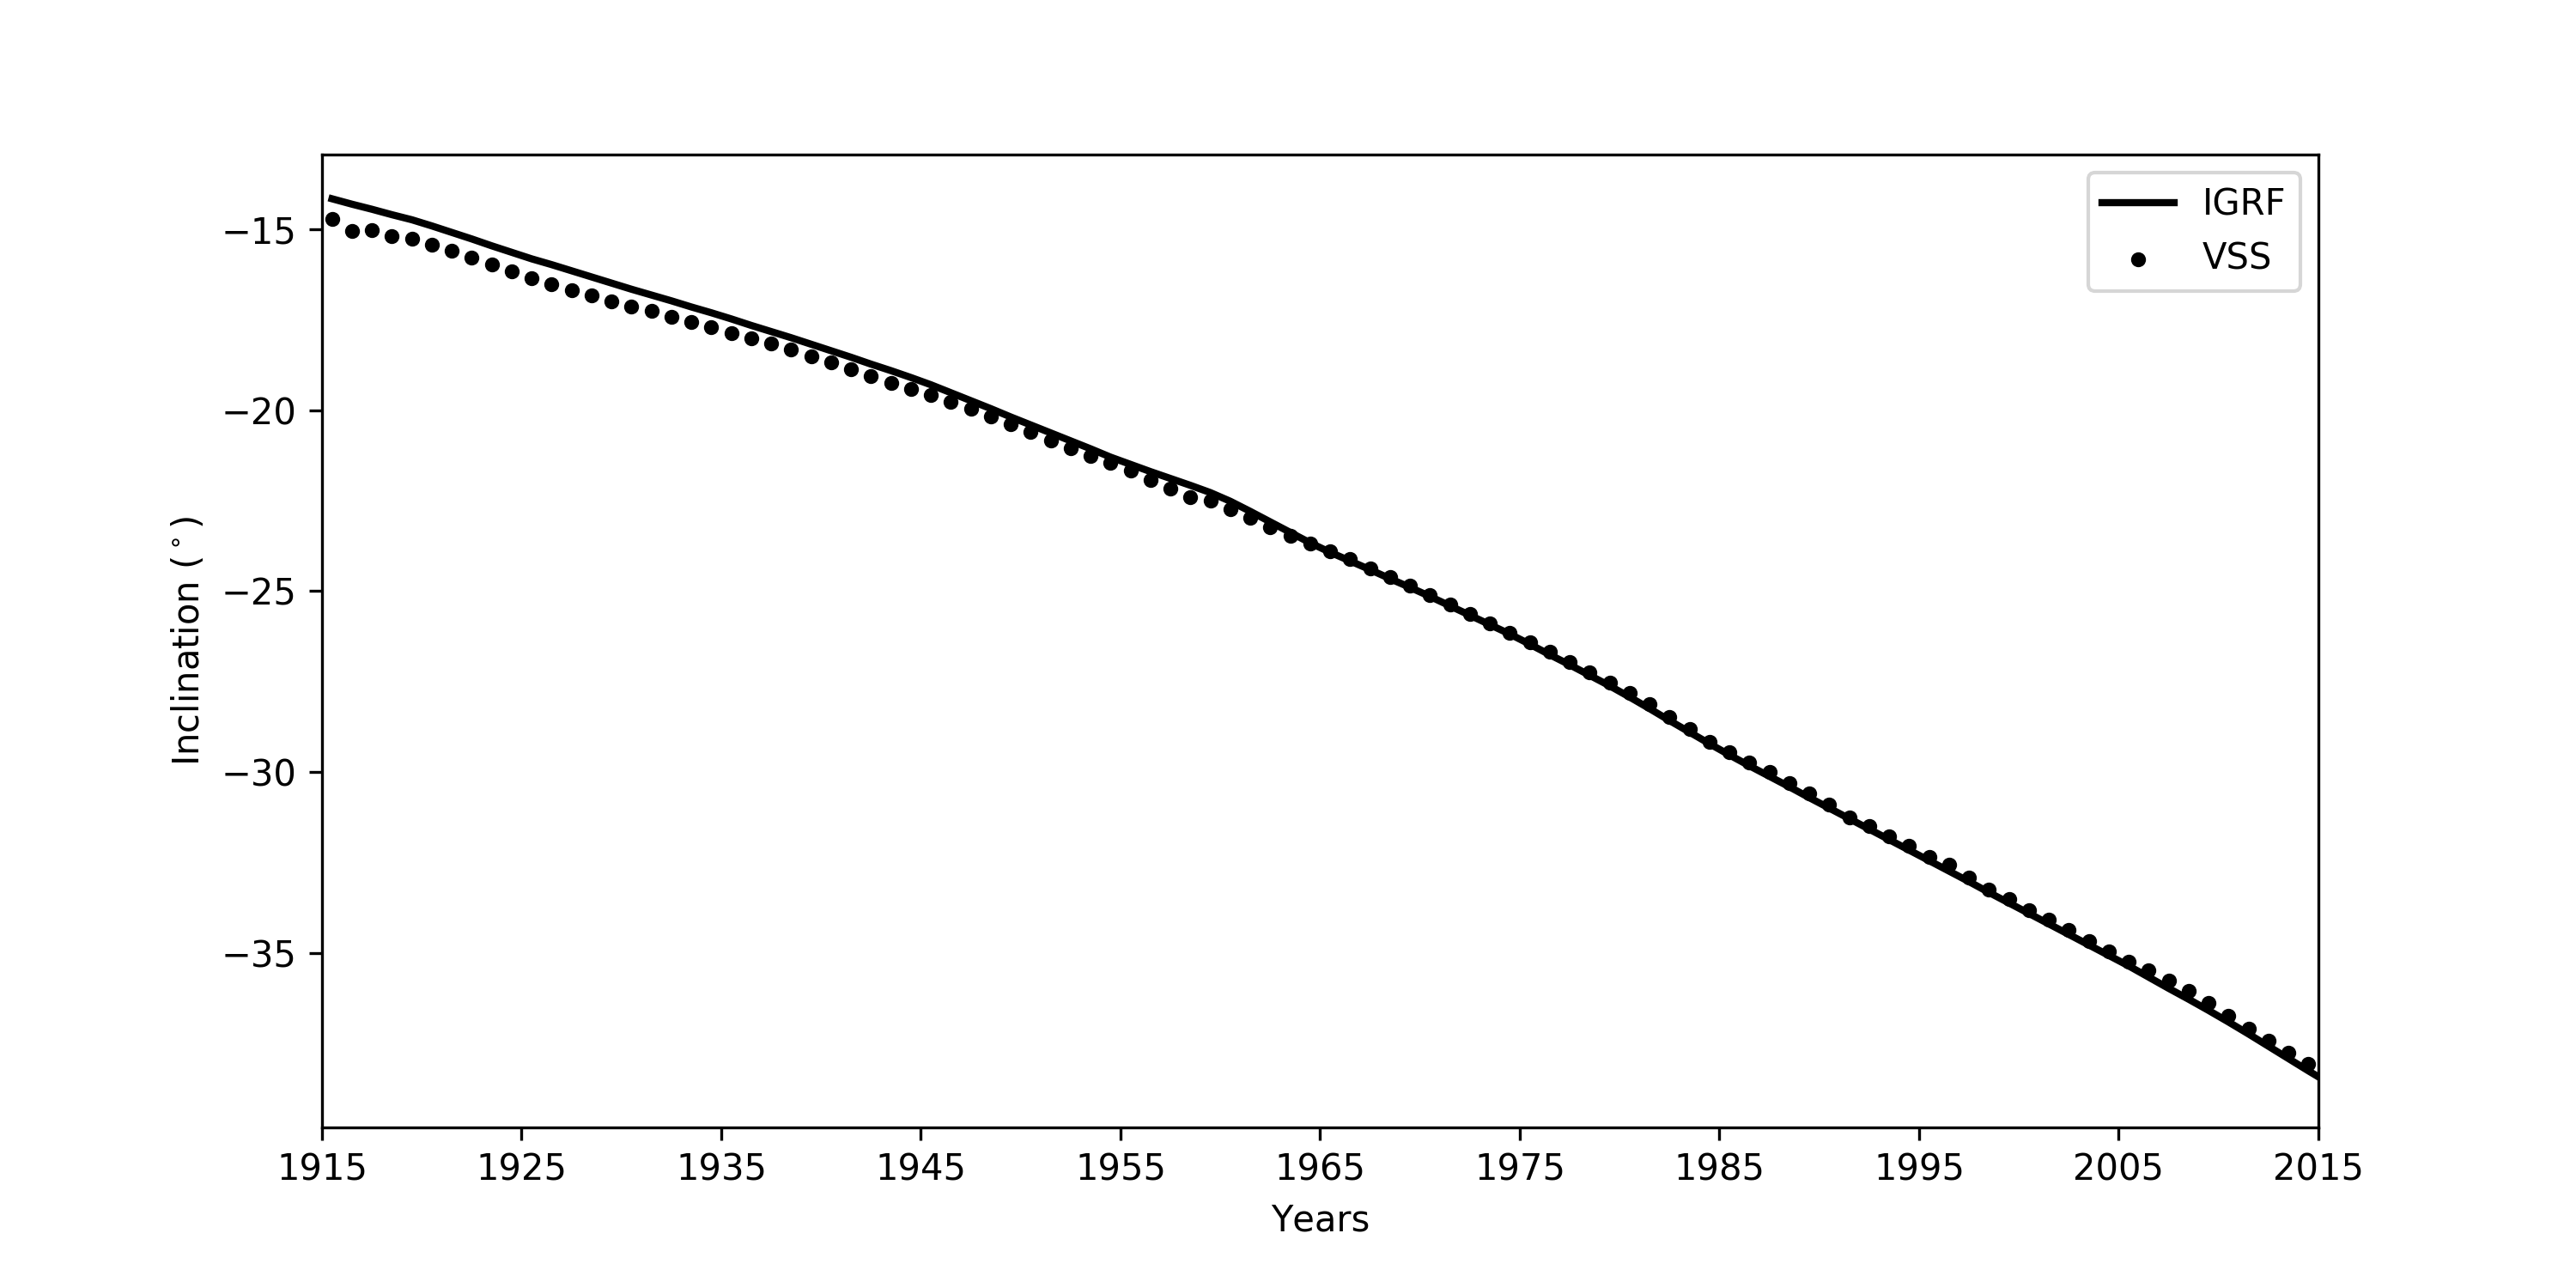
\includegraphics[width=1.0\linewidth]{I}
%	\caption{6. RMS (Declination) = 1.88 (\%)}
%	\label{ico}
%\end{figure}


%	\begin{figure}
%		\centering
%		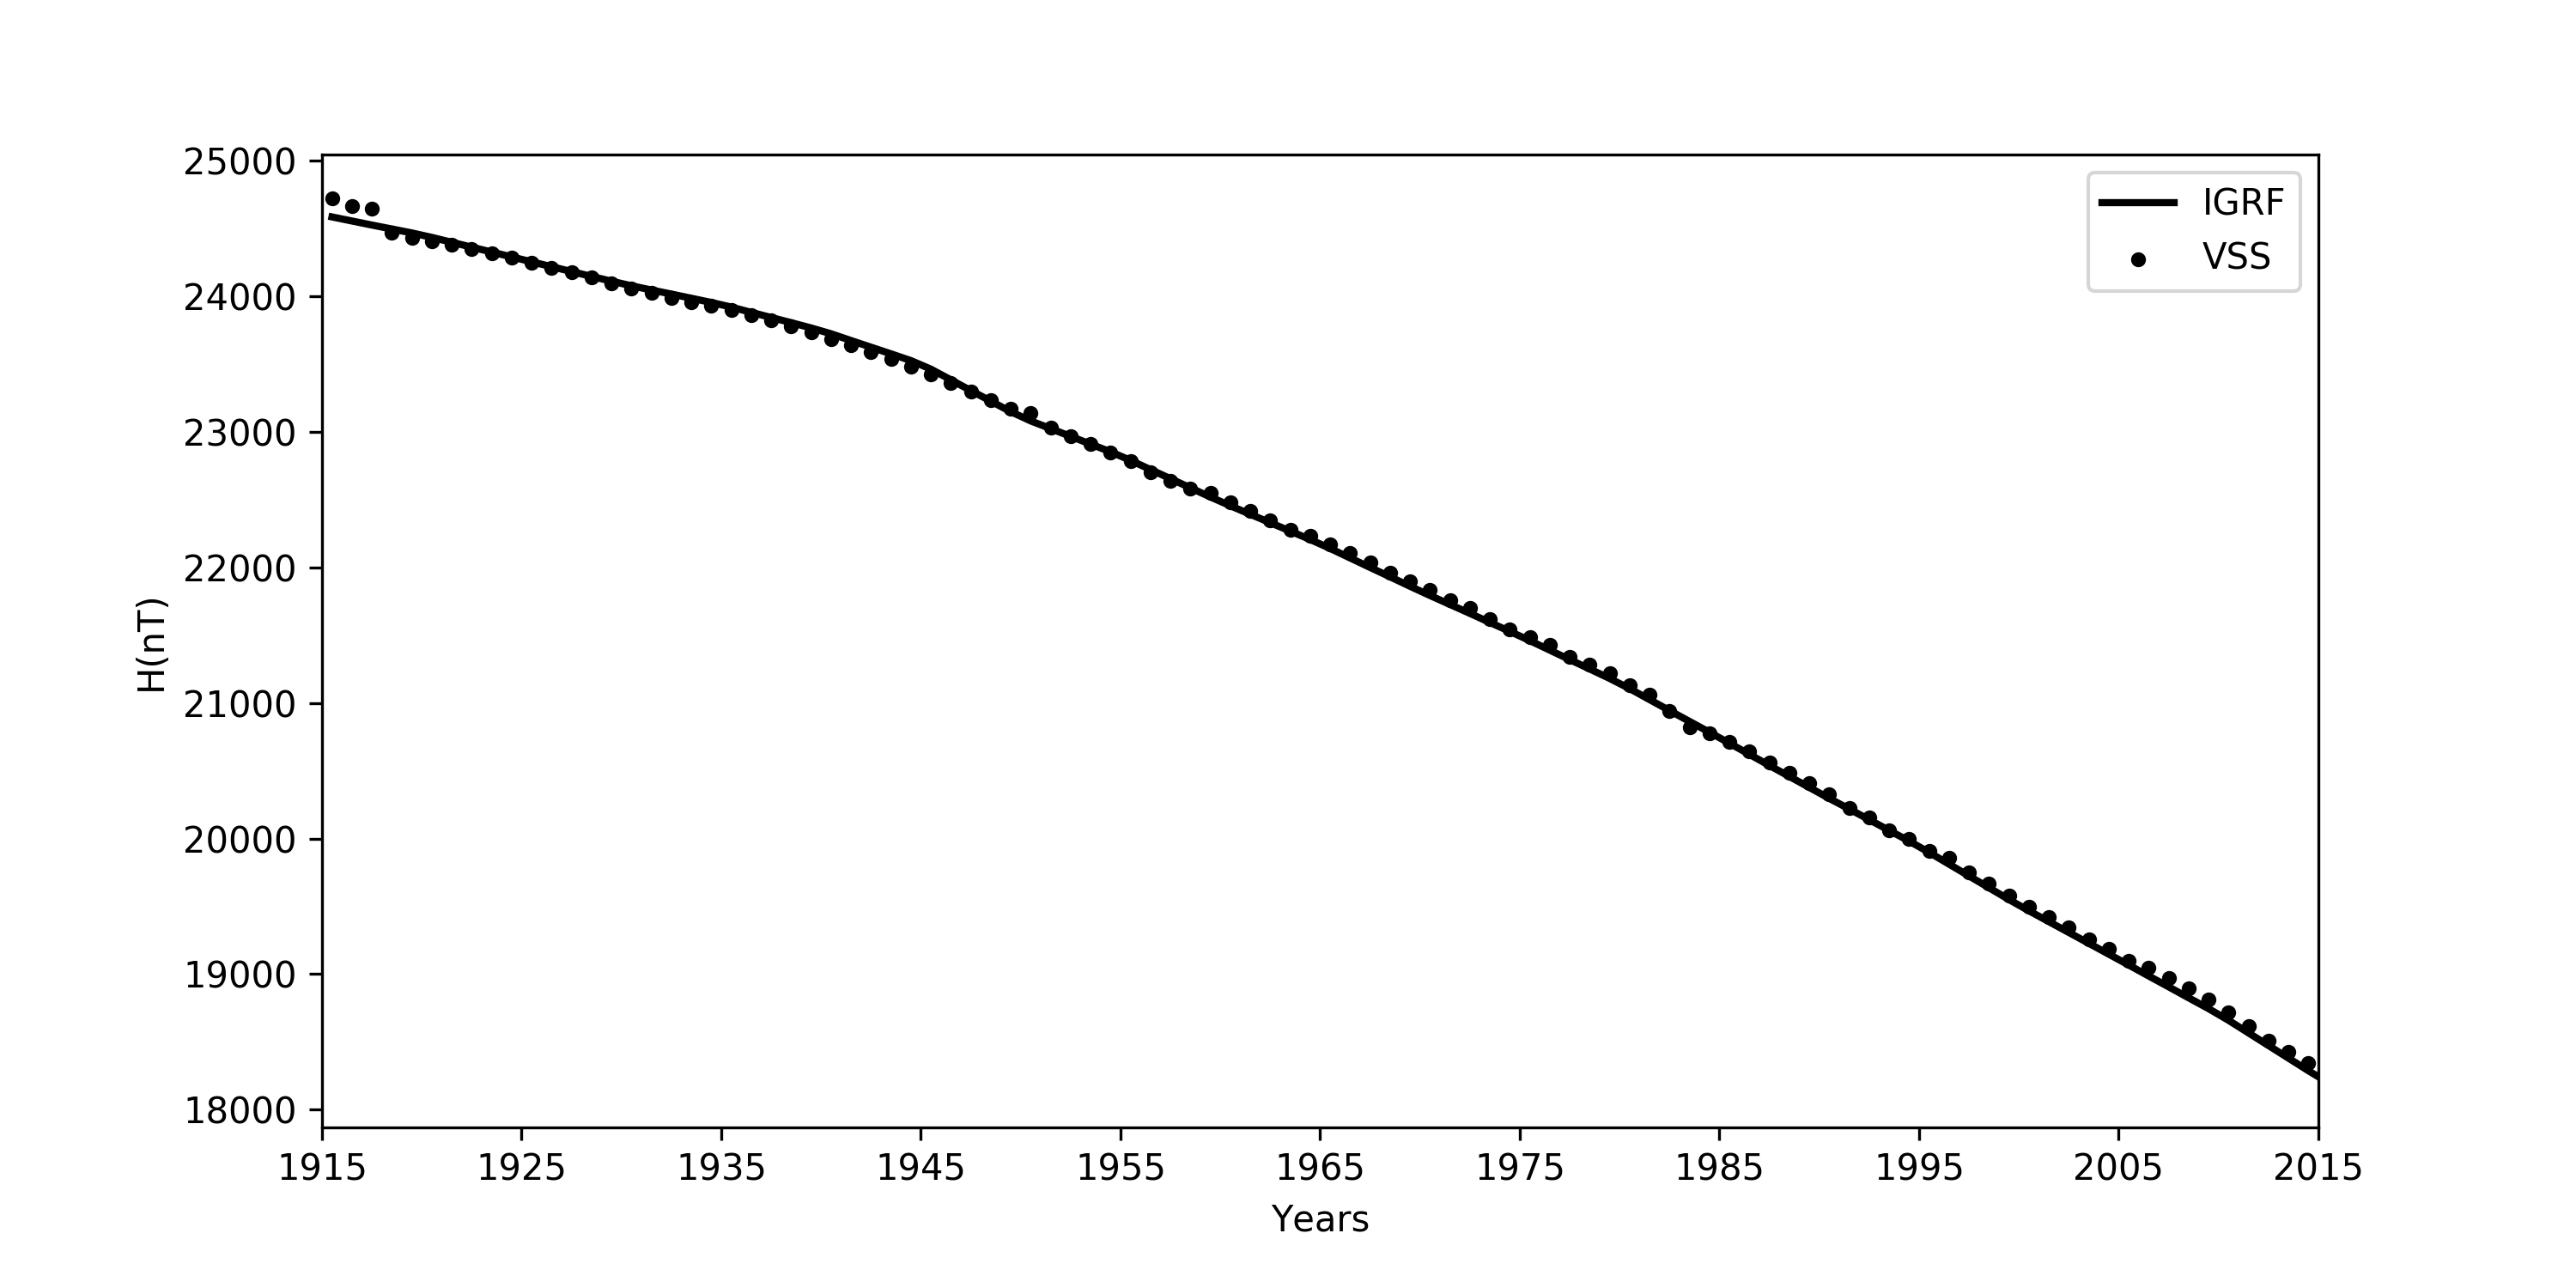
\includegraphics[width=1.0\linewidth]{H}
%		\caption{7. RMS (H component) = 1.98 (\%)}
%		\label{f_Sintetico}
%	\end{figure}

